\documentclass[10pt]{article}
\usepackage{graphicx}
\usepackage{colortbl}
\usepackage{amssymb}
\usepackage{float}
\usepackage{color}
\usepackage{tikz}
\usepackage{epstopdf}
\usepackage{enumitem}
\usepackage{multicol,multirow}
\DeclareGraphicsRule{.tif}{png}{.png}{`convert #1 `dirname #1`/`basename #1 .tif`.png}
\renewcommand{\tablename}{Tabla} 
\renewcommand{\figurename}{Figura} 
\newcommand*\circled[1]{\tikz[baseline=(char.base)]{\node[shape=circle,blue,draw,inner sep=2pt] (char) {#1};}}

\usepackage{listings}

\definecolor{mygreen}{rgb}{0,0.6,0}
\definecolor{mygray}{rgb}{0.5,0.5,0.5}
\definecolor{mymauve}{rgb}{0.58,0,0.82}


\lstset{ %
  backgroundcolor=\color{white},   % choose the background color; you must add \usepackage{color} or \usepackage{xcolor}
  basicstyle=\footnotesize,        % the size of the fonts that are used for the code
  breakatwhitespace=false,         % sets if automatic breaks should only happen at whitespace
  breaklines=true,                 % sets automatic line breaking
  captionpos=b,                    % sets the caption-position to bottom
  commentstyle=\color{gray},       % comment style
  deletekeywords={...},            % if you want to delete keywords from the given language
  escapeinside={\%*}{*)},          % if you want to add LaTeX within your code
  extendedchars=true,              % lets you use non-ASCII characters; for 8-bits encodings only, does not work with UTF-8
  frame=none,	                   % adds a frame around the code
  keepspaces=true,                 % keeps spaces in text, useful for keeping indentation of code (possibly needs columns=flexible)
  keywordstyle=\color{blue},       % keyword style
  language=Java,                 % the language of the code
  otherkeywords={else,open},           % if you want to add more keywords to the set
  numbers=left,                    % where to put the line-numbers; possible values are (none, left, right)
  numbersep=20pt,                   % how far the line-numbers are from the code
  numberstyle=\color{mygray}, % the style that is used for the line-numbers
  rulecolor=\color{black},         % if not set, the frame-color may be changed on line-breaks within not-black text (e.g. comments (green here))
  showspaces=false,                % show spaces everywhere adding particular underscores; it overrides 'showstringspaces'
  showstringspaces=false,          % underline spaces within strings only
  showtabs=false,                  % show tabs within strings adding particular underscores
  stepnumber=2,                    % the step between two line-numbers. If it's 1, each line will be numbered
  stringstyle=\color{mymauve},     % string literal style
  tabsize=2,	                   % sets default tabsize to 2 spaces
  title=\lstname                   % show the filename of files included with \lstinputlisting; also try caption instead of title
}


% For a visual definition of these parameters, see
\textwidth = 6.5 in
\textheight = 9 in
\oddsidemargin = 0.0 in
\evensidemargin = 0.0 in
\topmargin = 0.0 in             
\headheight = 0.0 in            
\headsep = 0.0 in
            
\parskip = 0.2in                % vertical space between paragraphs
% Delete the % in the following line if you don't want to have the first line of every paragraph indented
%\parindent = 0.0in

\begin{document}
\begin{center}
    {\Large Pauta Certamen 3, Programaci\'on II} \\
    %\emph{\small Prof. Rodrigo Olivares} \\
    %\emph{\scriptsize Junio 29, 2017}
\end{center}
\vspace*{-35pt}
\begin{center}
    \rule{1\textwidth}{.3pt}
\end{center}
\vspace*{-42pt}
\begin{center}
    \rule{1\textwidth}{2pt}
\end{center}

%\vspace*{-15pt}
%{\small \textbf{Instrucciones}:}
%\vspace*{-15pt}
%
{\scriptsize
%\begin{itemize}
%    \item[-] El puntaje m\'aximo del certamen es 100\%, siendo el 60\% el m\'inimo requerido para aprobar.
%    \item[-] Responda seg\'un las indicaciones dadas.
%    \item[-] El certamen es \underline{\textbf{individual}}. Cualquier intento de copia, ser\'a sancionado con nota \textbf{1,0}.
%\end{itemize}
%\vspace*{10pt}
%
%\vspace*{-30pt}

\begin{enumerate}

    \item \emph{30pts.} De las siguentes afirmaciones, encierre en un c\'irculo la o las alternativas correctas. Pueden ser todas, algunas, una o ninguna [60 minutos].
    \begin{multicols}{2}

    \begin{enumerate}[label=(\alph*)]
        \item[i.] \emph{3pts.} Respecto a las interfaces gr\'aficas en Java:
        \item Swing sustituye a AWT.
        \item AWT sustituye a Swing.
        \item AWT se apoya en Swing.
        \item AWT incopora los JComponents.
        \item Swing proporciona los ActionEvent.
    \end{enumerate}

    \begin{enumerate}[label=(\alph*)]
        \item[ii.] \emph{4pts.} Referente a JFrame:
        \item[\circled{(a)}] Habitualmente se usa para crear la ventana principal.
        \item[(b)] Su m\'etodo getPaneContent() obtiene el panel principal.
        \item[\circled{(c)}] Su m\'etodo add() permite agregar componentes al panel.
        \item[(d)] Su m\'etodo size() permite dimensionar la ventana.
        \item[(e)] Su m\'etodo pack() empaqueta las clases.
    \end{enumerate}

    \begin{enumerate}[label=(\alph*)]
        \item[iii.] \emph{4pts.} Continuando con JFrame:
        \item[(a)] Es posible implementarlo.
        \item[\circled{(b)}] Es posible extenderlo.
        \item[\circled{(c)}] Es posible instanciarlo.
        \item[(d)] Incluye el atributo est\'atico CLOSE\_AND\_EXIT.
        \item[\circled{(e)}] Incluye el m\'etodo setVisible(boolean).
    \end{enumerate}

    \begin{enumerate}[label=(\alph*)]
        \item[iv.] \emph{4pts.} Para realizar acciones desde un bot\'on, se requiere:
        \item[(a)] Crear una clase que implemente un ActionEvent.
        \item[(b)] Crear una clase que implemente un ActionList.
        \item[(c)] Sobreescribir el m\'etodo actionList(ActionPerformance)
        \item[(d)] Sobreescribir el m\'etodo actionArrayList(ActionEvent)
        \item[\circled{(e)}] Agregar la instancia que implementa un ActionListener.
    \end{enumerate}
    
    \begin{enumerate}[label=(\alph*)]
        \item[v.] \emph{3pts.} Algunos JComponents : 
        \item[(a)] JPane, JScrollPane, JDialog.
        \item[(b)] JPanel, JScrollPanel, JDialogPane.
        \item[\circled{(c)}] JFileChooser, JScrollPane, JLabel.
        \item[(d)] JCheckRadio, JTextArea, JText.
        \item[(e)] JDialogPane, JTextField, JTextArea.
    \end{enumerate}

    \begin{enumerate}[label=(\alph*)]
        \item[vi.] \emph{4pts.} Sobre los BorderLayout: 
        \item[(a)] Cada regi\'on se ordena GridLayout.
        \item[(b)] Cada regi\'on es obligatoria.
        \item[\circled{(c)}] Su constructor recibe argumentos de margen.
        \item[(d)] Agrega un panel en cada regi\'on.
        \item[(e)] setFlowLayout(boolean) fija una nueva dispoci\'on.
    \end{enumerate}

    \begin{enumerate}[label=(\alph*)]
        \item[vii.] \emph{4pts.} Sobre los JCheckbox: 
        \item[\circled{(a)}] Al pulsarse, cambia de estado.
        \item[(b)] Es una especializaci\'on del JButton.
        \item[\circled{(c)}] Al ser un bot\'on, tambien puede escuchar acciones.
        \item[\circled{(d)}] El m\'etodo isSelected() entrega su estado.
        \item[(e)] S\'olo se puede seleccionar uno de un grupo.
    \end{enumerate}

    \begin{enumerate}[label=(\alph*)]
        \item[viii.] \emph{4pts.} Sobre los JLabel: 
        \item[\circled{(a)}] Su constructor recibe texto.
        \item[\circled{(b)}] Su constructor recibe im\'agenes.
        \item[\circled{(c)}] Su constructor recibe texto e im\'agenes, al mismo tiempo.
        \item[(d)] Su constructor recibe el tama\~no del texto a mostrar.
        \item[(e)] No pueden ser modificados en ejecuci\'on.
    \end{enumerate}

\end{multicols}

\newpage

\item \emph{70pts.} Desarrolle el juego ``El Gato''. Se pide lo siguiente:

\begin{itemize}
    \item Al iniciar el sistema, se debe deplegar el siguiente mensaje:
    
    \begin{figure}[H]
        \begin{center}
            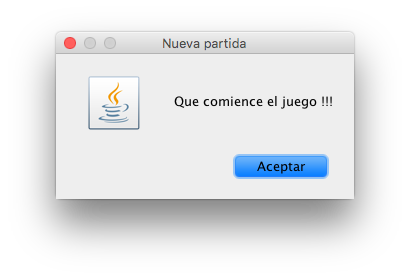
\includegraphics[scale=.5]{img_msg_inicio.png}
        \end{center}
    \end{figure}
   
    \item Al presionar aceptar, se despliega el tablero vac\'io:
    
    \begin{figure}[H]
        \begin{center}
            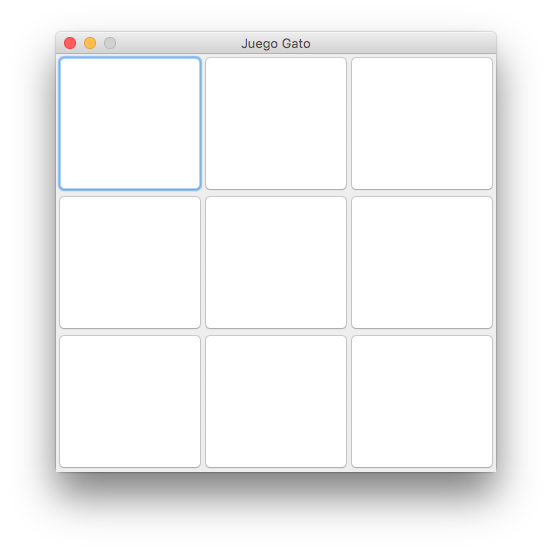
\includegraphics[scale=.5]{img_inicio.png}
        \end{center}
    \end{figure}
    
    \item El jugardor siempre comienza jugando.

    \item La selecci\'on de \textbf{cruz} y \textbf{c\'irculo} debe ser al azar, para el jugador y la m\'aquina.

    \item Al presionar en una casilla, \'esta se selecciona y se bloquea. En ese instante, la m\'aquina selecciona al \textbf{azar} una casilla libre (no bloqueada):
    
    \begin{figure}[H]
        \begin{center}
            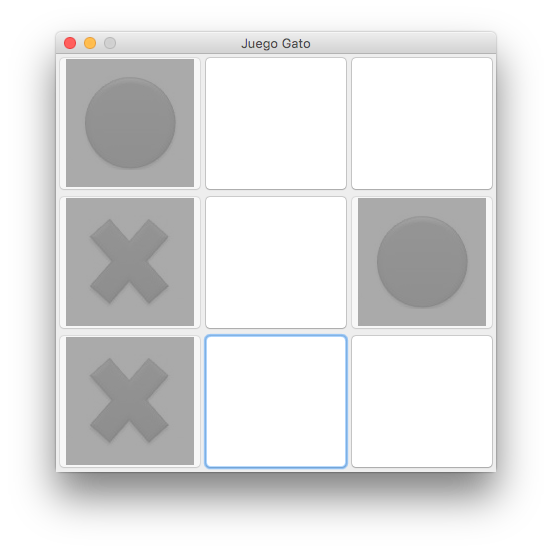
\includegraphics[scale=.5]{img_juego.png}
        \end{center}
    \end{figure}
    
    \item Si el jugador obtiene 3 selecciones en l\'inea (horizontal, recta, diagonal derecha o diagonal izquierda), gana. Se debe informar que el jugador ha ganado la partida.
    
    \begin{figure}[H]
        \begin{center}
            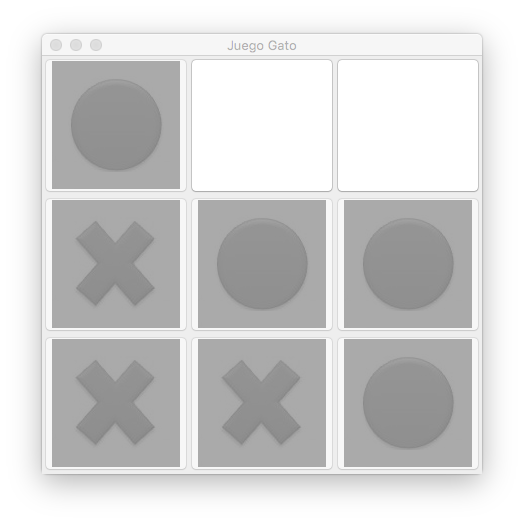
\includegraphics[scale=.5]{img_gano.png}
        \end{center}
    \end{figure}

    \begin{figure}[H]
        \begin{center}
            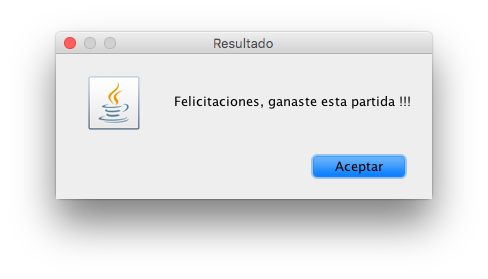
\includegraphics[scale=.5]{img_msg_gano.png}
        \end{center}
    \end{figure} 
    
    \item Si la m\'aquina obtiene 3 selecciones en l\'inea (horizontal, recta, diagonal derecha o diagonal izquierda), ud pierde. Se debe informar que la m\'aquina ha ganado la partida.
    
    \begin{figure}[H]
        \begin{center}
            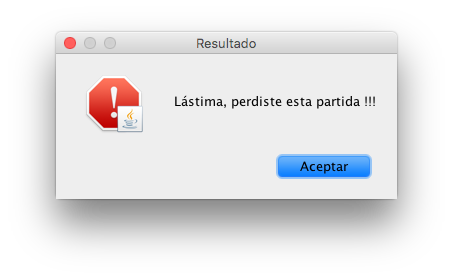
\includegraphics[scale=.5]{img_msg_perdio.png}
        \end{center}
    \end{figure} 
    
    \item Si hay empate, el sistema debe desplegar el siguiente mensaje:
    
        \begin{figure}[H]
        \begin{center}
            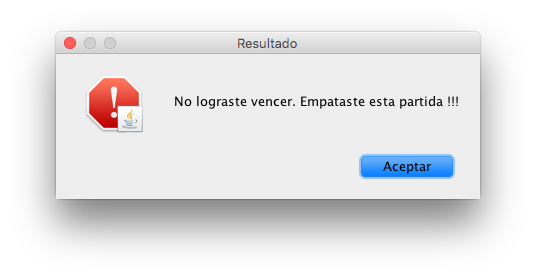
\includegraphics[scale=.5]{img_msg_empate.png}
        \end{center}
    \end{figure}     
     
\end{itemize}

 \newpage

\lstinputlisting[numbers=none,caption=]{java/JuegoVentana.java} 

\end{enumerate}
}
\end{document} 
